\documentclass{article}

\usepackage{graphicx}

\title{Chat application report}
\author{Abdun Nihaal}

\begin{document}
\maketitle

\section{Introduction}

The objective set by this assignment is to create a chat application using java that enables users to send messages to other users one on one or in a group.

\section{Design}

\subsection{One thread per client architecture}

In this chat server architecture, whenever a client connects to the server, the server creates a separate thread to handle the client.
The problem with this architecture is that it may create more threads than what the server CPU cores can handle.
Context switching between threads can be expensive and take a lot of memory.
In this architecture, the threads perform blocking reads and writes with the client.

\subsection{Selector based non-blocking server architecture}

Java Nio's selector class can manage multiple channels from a single thread. 
With the use of Java Nio's selector class, this server does non blocking IO when reading or writing to the client.

\begin{figure}
	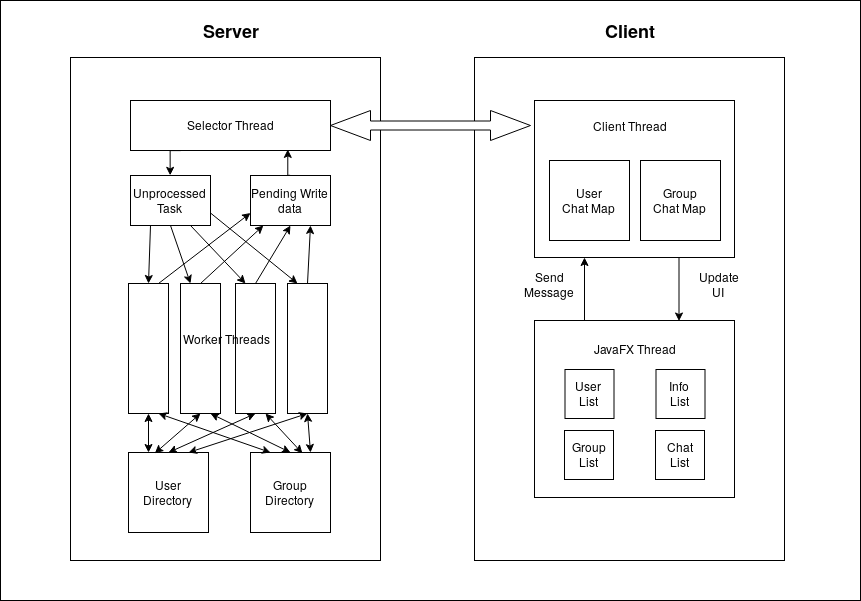
\includegraphics[width=\linewidth]{architecture.png}
	\caption{Chat server architecture}
	\label{fig:architecture}
\end{figure}

The Chat Server Architecture is shown in fig. \ref{fig:architecture}. The server consists of a selector thread and a number of worker threads.
The selector thread is responsible for performing network IO and reacting to events. The worker threads process the messages that are received by the selector thread.
This architecture enables the worker threads to share the workload.

The communication between the selector and worker threads is achieved by using two data structures. UnprocessedTask queue is a queue of messages that were received by the selector thread. 
When a worker thread is free, it retrieves a message from the UnprocessedTask queue and processes it.
When the worker wants to send a message to a client, it adds the message to the PendingWrite queue. 
The selector thread writes the data from PendingWrite queue to the corresponding socket channel.

The server maintains a user directory and a group directory. 
The user directory keeps track of all the online users. 
It stores the username and their corresponding SelectionKey which can be used to send and receive messages from the user's client.

The group directory contains a list of groups created and the users who are present in that group. Whenever a group message is received, the server retrieves the list of users in that group and sends the message to all of them.

Messages are processed using string patterns.
Messages exchanged between the server and the client are of the form

COMMAND\$arg1\$arg2\$...\#\#

Some of the message types used are

\begin{itemize}
	\item LOGIN\$username\#\#

		When this message is sent to the server, the server tries to log the user in with the given username

	\item MSG\$ReciverName\$Message\#\#

		This is sent by the client if it wants to send the message to receiver denoted by ReceiverName
	\item GMSG\$GroupName\$Message\#\#

		This is sent by the client if it wants to send a group message to the group denoted by GroupName

	\item GCREATE\$GroupName\#\#

		This creates a group with the group name given and adds the user as a member of the group

	\item GADD\$GroupName\$list,of,users\#\#

		This adds the users present in the list of users to the group given by the group name

	\item GDELETE\$GroupName\#\#

		This deletes the group given by the GroupName

	\item LOGOUT\#\#

		This logs the user out. The server deletes the user from the user directory
\end{itemize}

\section{Analysis}

The response time of the server was measured using a java program that creates a given number of client threads. Each client thread simultaneously sends 10000 echo message i.e. it sends a random string as a message to itself and measures the average time between sending and receiving the message.

In fig. \ref{fig:responsetime}, the different lines show the response times for different number of client threads. 
While performing analysis the client and the server threads were run on the same computer so the improvement when using more threads is countered by the switching of threads.
We can see a slight decrease in response time when using multiple worker threads when the number of clients are more.

\begin{figure}
	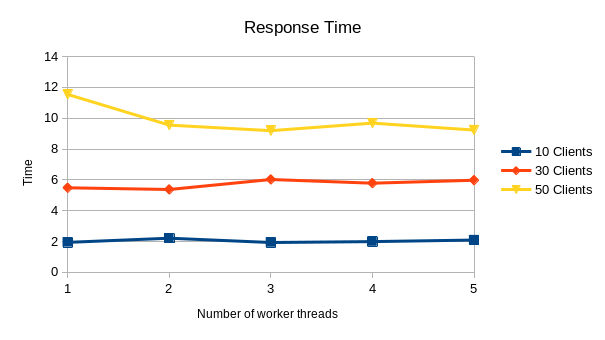
\includegraphics[width=\linewidth]{responsetime.png}
	\caption{Response Time}
	\label{fig:responsetime}
\end{figure}

\section{Conclusion}

Thus the Chat server for P2P and group chat is implemented using Java Nio and the client application is implemented using JavaFx and Java Nio.

\end{document}
